\begin{aosachapter}{A Continuous Integration System}{s:ci}{Malini Das}

\aosasecti{What is a Continuous Integration
System?}\label{what-is-a-continuous-integration-system}

When developing software, we want to be able to verify that our new
features or bug fixes are safe and work as expected. We do this by
running tests against our code. Sometimes, developers will run tests
locally to verify that their changes are safe, but developers may not
have the time to test their code on every system their software runs in.
Further, as more and more tests are added the amount of time required to
run them, even only locally, becomes less viable. Because of this,
continuous integration systems have been created.

Continuous Integration (CI) systems are dedicated systems used to test
new code. Upon a commit to the code repository, it is the responsibility
of the continuous integration system to verify that this commit will not
break any tests. To do this, the system must be able to fetch the new
changes, run the tests and report its results. Like any other system, it
should also be failure resistant. This means if any part of the system
fails, it should be able to recover and continue from that point.

This test system should also handle load well, so that we can get test
results in a reasonable amount of time in the event that commits are
being made faster than the tests can be run. We can achieve this by
distributing and parallelizing the testing effort. This project will
demonstrate a small-scale, distributed continuous integration system. It
is a bare-bones system, but is designed for extensibility.

\aosasecti{Project Limitations and
Notes}\label{project-limitations-and-notes}

This project uses Git as the repository for the code that needs to be
tested. Only standard source code management calls will be used, so if
you are unfamiliar with Git but are familiar with other version control
systems (VCS) like svn or Mercurial, you can still follow along.

This project also assumes you are using a POSIX system.

Due to the limitations of code length and unittest, I simplified test
discovery. We will \emph{only} run tests that are in a directory named
\texttt{tests} within the repository.

Continuous integration systems monitor a master repository which is
usually hosted on a web server, and not local to the CI's file systems.
For the cases of our example, we will use a local repository instead of
a remote repository.

Continuous integration systems need not run on a fixed, regular
schedule. You can also have them run every few commits, or per-commit.
For our example case, the CI system will run periodically. This means if
it is set up to check for changes in five-second periods, it will run
tests against the most recent commit made after the five-second period.
It won't test every commit made within that period of time, only the
most recent one.

This CI system is designed to check periodically for changes in a
repository. In real-world CI systems, you can also have the repository
observer get notified by a hosted repository. Github, for example,
provides ``post-commit hooks'' which send out notifications to a URL.
Following this model, the repository observer would be called by the web
server hosted at that URL to respond to that notification. Since this is
complex to model locally, we're using an observer model, where the
repository observer will check for changes instead of being notified.

CI systems also have a reporter aspect, where the test runner reports
its results to a component that makes them available for people to see,
perhaps on a webpage. For simplicity, this project gathers the test
results and stores them as files in the file system local to the
dispatcher process.

Note that the architecture this CI system uses is just one possibility
among many. This approach has been chosen to simplify our case study
into three main components.

\aosasecti{Introduction}\label{introduction}

The basic structure of a continuous integration system consists of three
components: an observer, a test job dispatcher, and a test runner. The
observer watches the repository. When it notices that a commit has been
made, it notifies the job dispatcher. The job dispatcher then finds a
test runner and gives it the commit number to test.

There are many ways to architect a CI system. We could have the
observer, dispatcher and runner be the same process on a single machine.
This approach is very limited since there is no load handling, so if
more changes are added to the repository than the CI system can handle,
a large backlog will accrue. This approach is also not fault-tolerant at
all; if the computer it is running on fails or there is a power outage,
there are no fallback systems, so no tests will run. The ideal system
would be one that can handle as many test jobs as requested, and will do
its best to compensate when machines go down.

To build a CI system that is fault-tolerant and load-bearing, in this
project, each of these components is its own process. This will let each
process be independent of the others, and let us run multiple instances
of each process. This is useful when you have more than one test job
that needs to be run at the same time. We can then spawn multiple test
runners in parallel, allowing us to run as many jobs as needed, and
prevent us from accumulating a backlog of queued tests.

In this project, not only do these components run as separate processes,
but they also communicate via sockets, which will let us run each
process on a separate, networked machine. A unique host/port address is
assigned to each component, and each process can communicate with the
others by posting messages at the assigned addresses.

This design will let us handle hardware failures on the fly by enabling
a distributed architecture. We can have the observer run on one machine,
the test job dispatcher on another, and the test runners on another, and
they can all communicate with each other over a network. If any of these
machines go down, we can schedule a new machine to go up on the network,
so the system becomes fail-safe.

This project does not include auto-recovery code, as that is dependent
on your distributed system's architecture, but in the real world, CI
systems are run in a distributed environment like this so they can have
failover redundancy (i.e., we can fall back to a standby machine if one
of the machines a process was running on becomes defunct).

For the purposes of this project, each of these processes will run
locally, and you must kick them off individually. Since the processes
need to communicate with each other, they will run on distinct local
ports.

\aosasectii{Files in this Project}\label{files-in-this-project}

This project contains Python files for each of these components: the
repository observer (\texttt{repo\_observer.py}), the test job
dispatcher (\texttt{dispatcher.py}), and the test runner
(\texttt{test\_runner.py}). Each of these three processes communicate
with each other using sockets, and since the code used to transmit
information is shared by all of them, there is a helpers.py file that
contains it, so each process imports the communicate function from here
instead of having it duplicated in the file.

There are also bash script files used by these processes. These script
files are used to execute bash and git commands in an easier way than
constantly using Python's operating system-level modules like os and
subprocess.

Lastly, there is a tests directory, which contains two example tests the
CI system will run. One test will pass, and the other will fail.

\aosasectii{Initial Setup}\label{initial-setup}

While this CI system is ready to work in a distributed system, let us
start by running everything locally on one computer so we can get a
grasp on how the CI system works without adding the risk of running into
network-related issues. If you wish to run this in a distributed
environment, you can run each component on its own machine.

Continuous integration systems run tests by detecting changes in a code
repository, so to start, we will need to set up the repository our CI
system will monitor.

Let's call this \texttt{test\_repo}:

\begin{verbatim}
$ mkdir test_repo 
$ cd test_repo 
$ git init
\end{verbatim}

This will be our master repository. This is where developers check in
their code, so our CI should pull this repository and check for commits,
then run tests. The thing that checks for new commits is the repository
observer.

The repository observer works by checking commits, so we need at least
one commit in the master repository. Let's commit our example tests so
we have some tests to run.

Copy the tests folder from this code base to \texttt{test\_repo} and
commit it:

\begin{verbatim}
$ cp -r /this/directory/tests /path/to/test_repo/ 
$ cd /path/to/test\_repo 
$ git add tests/ 
$ git commit -m”add tests”
\end{verbatim}

Now you have a commit in the master repository.

The repo observer component will need its own clone of the code, so it
can detect when a new commit is made. Let's create a clone of our master
repository, and call it \texttt{test\_repo\_clone\_obs}:

\begin{verbatim}
$ git clone /path/to/test_repo test_repo_clone_obs
\end{verbatim}

The test runner will also need its own clone of the code, so it can
checkout the repository at a given commit and run the tests. Let's
create another clone of our master repository, and call it
\texttt{test\_repo\_clone\_runner}:

\begin{verbatim}
$ git clone /path/to/test_repo test_repo_clone_runner
\end{verbatim}

\aosasecti{The Components}\label{the-components}

\aosasectii{The Repository Observer
(\texttt{repo\_observer.py})}\label{the-repository-observer-repoux5fobserver.py}

The repository observer monitors a repository and notifies the
dispatcher when a new commit is seen. In order to work with all version
control systems (since not all VCSs have built-in notification systems),
this repository observer is written to periodically check the repository
for new commits instead of relying on the VCS to notify it that changes
have been made.

The observer will poll the repository periodically, and when a change is
seen, it will tell the dispatcher the newest commit ID to run tests
against. The observer checks for new commits by finding the current
commit ID in its repository, then updates the repository, and lastly, it
finds the latest commit ID and compares them. For the purposes of this
example, the observer will only dispatch tests against the latest
commit. This means that if two commits are made between a periodic
check, the observer will only run tests against the latest commit.
Usually, a CI system will detect all commits since the last tested
commit, and will dispatch test runners for each new commit, but I have
modified this assumption for simplicity.

The observer must know which repository to observe. We previously
created a clone of our repository at
\texttt{/path/to/test\_repo\_clone\_obs}. The repository will use this
clone to detect changes. To allow the repository observer to use this
clone, we pass it the path when we invoke the \texttt{repo\_observer.py}
file. The repository observer will use this clone to pull from the main
repository.

We must also give the observer the dispatcher's address, so the observer
may send it messages. When you start the repository observer, you can
pass in the dispatcher's server address using the
\texttt{-{}-dispatcher-server} command line argument. If you do not pass
it in, it will assume the default address of \texttt{localhost:8888}.

\begin{verbatim}
def poll():
    parser = argparse.ArgumentParser()
    parser.add_argument("--dispatcher-server",
                        help="dispatcher host:port, " \
                        "by default it uses localhost:8888",
                        default="localhost:8888",
                        action="store")
    parser.add_argument("repo", metavar="REPO", type=str,
                        help="path to the repository this will observe")
    args = parser.parse_args()
    dispatcher_host, dispatcher_port = args.dispatcher_server.split(":")
\end{verbatim}

Once the repository observer file is invoked, it starts the
\texttt{poll()} function. This function parses the command line
arguments, and then kicks off an infinite while loop. The while loop is
used to periodically check the repository for changes. The first thing
it does is call the \texttt{update\_repo.sh} Bash script. (Bash is used
because we need to check file existence, create files, and use Git, and
a shell script is the most direct and easy way to achieve this.
Alternatively, there are cross-platform Python packages you can use; for
example, Python's \texttt{os} built-in module can be used for accessing
the file system, and GitPython can be used for Git access, but they
perform actions in a more roundabout way.)

\begin{verbatim}
    while True:
        try:
            # call the bash script that will update the repo and check
            # for changes. If there's a change, it will drop a .commit_id file
            # with the latest commit in the current working directory
            subprocess.check_output(["./update_repo.sh", args.repo])
        except subprocess.CalledProcessError as e:
            raise Exception("Could not update and check repository. Reason: %s" % e.output)
\end{verbatim}

The \texttt{update\_repo.sh} file is used to identify any new commits
and let the repository observer know. It does this by noting what commit
ID we are currently aware of, then pulls the repository, and checks the
latest commit ID. If they match, no changes are made, so the repository
observer doesn't need to do anything, but if there is a difference in
the commit ID, then we know a new commit has been made. In this case,
\texttt{update\_repo.sh} will create a file called \texttt{.commit\_id}
with the latest commit ID stored in it.

A step-by-step breakdown of \texttt{update\_repo.sh} is as follows.
First, the script sources the \texttt{run\_or\_fail.sh} file, which
provides the \texttt{run\_or\_fail} helper method used by all our shell
scripts. This method is used to run the given command, or fail with the
given error message.

\begin{verbatim}
#!/bin/bash

source run_or_fail.sh 
\end{verbatim}

Next, the script tries to remove a file named \texttt{.commit\_id}.
Since \texttt{updaterepo.sh} is called infinitely by the
\texttt{repo\_observer.py} file, if we previously had a new commit, then
\texttt{.commit\_id} was created, but holds a commit we already tested.
Therefore, we want to remove that file, and create a new one only if a
new commit is found.

\begin{verbatim}
bash rm -f .commit_id 
\end{verbatim}

After it removes the file (if it existed), it verifies that the
repository we are observing exists, and then resets it to the most
recent commit, in case anything caused it to get out of sync.

\begin{verbatim}
run_or_fail "Repository folder not found!" pushd $1 1> /dev/null
run_or_fail "Could not reset git" git reset --hard HEAD
\end{verbatim}

It then calls git log and parses the output, looking for the most recent
commit ID.

\begin{verbatim}
COMMIT=$(run_or_fail "Could not call 'git log' on repository" git log -n1)
if [ $? != 0 ]; then
  echo "Could not call 'git log' on repository"
  exit 1
fi
COMMIT_ID=`echo $COMMIT | awk '{ print $2 }'`
\end{verbatim}

Then it pulls the repository, getting any recent changes, then gets the
most recent commit ID.

\begin{verbatim}
run_or_fail "Could not pull from repository" git pull
COMMIT=$(run_or_fail "Could not call 'git log' on repository" git log -n1)
if [ $? != 0 ]; then
  echo "Could not call 'git log' on repository"
  exit 1
fi
NEW_COMMIT_ID=`echo $COMMIT | awk '{ print $2 }'`
\end{verbatim}

Lastly, if the commit ID doesn't match the previous ID, then we know we
have new commits to check, so the script stores the latest commit ID in
a .commit\_id file.

\begin{verbatim}
# if the id changed, then write it to a file
if [ $NEW_COMMIT_ID != $COMMIT_ID ]; then
  popd 1> /dev/null
  echo $NEW_COMMIT_ID > .commit_id
fi
\end{verbatim}

When \texttt{update\_repo.sh} finishes running in
\texttt{repo\_observer.py}, the repository observer checks for the
existence of the \texttt{.commit\_id} file. If the file does exist, then
we know we have a new commit, and we need to notify the dispatcher so it
can kick off the tests. The repository observer will check the
dispatcher server's status by connecting to it and sending a `status'
request, to make sure there are no problems with it, and to make sure it
is ready for instruction.

\begin{verbatim}
        if os.path.isfile(".commit_id"):
            try:
                response = helpers.communicate(dispatcher_host,
                                               int(dispatcher_port),
                                               "status")
            except socket.error as e:
                raise Exception("Could not communicate with dispatcher server: %s" % e)
\end{verbatim}

If it responds with ``OK'', then the repository observer opens the
\texttt{.commit\_id} file, reads the latest commit ID and sends that ID
to the dispatcher, using a
\texttt{dispatch:\textless{}commit ID\textgreater{}} request. It will
then sleep for five seconds and repeat the process. We'll also try again
in five seconds if anything went wrong along the way.

\begin{verbatim}
            if response == "OK":
                commit = ""
                with open(".commit_id", "r") as f:
                    commit = f.readline()
                response = helpers.communicate(dispatcher_host,
                                               int(dispatcher_port),
                                               "dispatch:%s" % commit)
                if response != "OK":
                    raise Exception("Could not dispatch the test: %s" %
                    response)
                print "dispatched!"
            else:
                raise Exception("Could not dispatch the test: %s" %
                response)
        time.sleep(5)
\end{verbatim}

The repository observer will repeat this process forever, until you kill
the process via a \texttt{KeyboardInterrupt} (Ctrl+c), or by sending it
a kill signal.

\aosasectii{The Dispatcher
(dispatcher.py)}\label{the-dispatcher-dispatcher.py}

The dispatcher is a separate service used to delegate testing tasks. It
listens on a port for requests from test runners and from the repository
observer. It allows test runners to register themselves, and when given
a commit ID from the repository observer, it will dispatch a test runner
against the new commit. It also gracefully handles any problems with the
test runners and will redistribute the commit ID to a new test runner if
anything goes wrong.

When dispatch.py is executed, the serve function is called. First it
parses the arguments that allow you to specify the dispatcher's host and
port:

``python def serve(): parser = argparse.ArgumentParser()
parser.add\_argument(``--host'', help=``dispatcher's host, by default it
uses localhost'', default=``localhost'', action=``store'')
parser.add\_argument(``--port'', help=``dispatcher's port, by default it
uses 8888'', default=8888, action=``store'') args = parser.parse\_args()

\begin{center}\rule{3in}{0.4pt}\end{center}

This starts the dispatcher server, and two other threads. One thread
runs the runner\_checker function, and other runs the redistribute
function.

\begin{aosadescription}
\item[``]
server = ThreadingTCPServer((args.host, int(args.port)),
DispatcherHandler) print serving on \%s:\%s \% (args.host,
int(args.port))

\ldots{}

runner\_heartbeat = threading.Thread(target=runner\_checker,
args=(server,)) redistributor = threading.Thread(target=redistribute,
args=(server,)) try: runner\_heartbeat.start() redistributor.start() \#
Activate the server; this will keep running until you \# interrupt the
program with Ctrl+C or Cmd+C server.serve\_forever() except
(KeyboardInterrupt, Exception): \# if any exception occurs, kill the
thread server.dead = True runner\_heartbeat.join() redistributor.join()
\end{aosadescription}

\begin{center}\rule{3in}{0.4pt}\end{center}

The runner\_checker function periodically pings each registered test
runner to make sure they are still responsive. If they become
unresponsive, then that runner will be removed from the pool and its
commit ID will be dispatched to the next available runner. The function
will log the commit ID in the pending\_commits variable.

\begin{aosadescription}
\item[``python]
\begin{aosadescription}
\item[def runner\_checker(server):]
\begin{aosadescription}
\item[def manage\_commit\_lists(runner):]
\begin{aosadescription}
\item[for commit, assigned\_runner in
server.dispatched\_commits.iteritems():]
\begin{aosadescription}

\item[if assigned\_runner == runner:]
del server.dispatched\_commits{[}commit{]}
server.pending\_commits.append(commit) break
\end{aosadescription}
\end{aosadescription}

server.runners.remove(runner)
\item[while not server.dead:]
time.sleep(1) for runner in server.runners: s =
socket.socket(socket.AF\_INET, socket.SOCK\_STREAM) try: response =
helpers.communicate(runner{[}``host''{]}, int(runner{[}``port''{]}),
``ping'') if response != ``pong'': print ``removing runner \%s'' \%
runner manage\_commit\_lists(runner) except socket.error as e:
manage\_commit\_lists(runner)
\end{aosadescription}
\end{aosadescription}
\end{aosadescription}

\begin{center}\rule{3in}{0.4pt}\end{center}

The redistribute function is used to dispatch the commit IDs logged in
pending\_commits. When redistribute runs, it checks if there are any
commit IDs in pending\_commits. If so, it calls the dispatch\_tests
function with the commit ID.

\begin{aosadescription}
\item[``python]
\begin{aosadescription}
\item[def redistribute(server):]
\begin{aosadescription}
\item[while not server.dead:]
\begin{aosadescription}

\item[for commit in server.pending\_commits:]
print ``running redistribute'' print server.pending\_commits
dispatch\_tests(server, commit) time.sleep(5)
\end{aosadescription}
\end{aosadescription}
\end{aosadescription}
\end{aosadescription}

\begin{center}\rule{3in}{0.4pt}\end{center}

The dispatch\_tests function is used to find an available test runner
from the pool of registered runners. If one is available, it will send a
runtest message to it with the commit ID. If none are currently
available, it will wait two seconds and repeat this process. Once
dispatched, it logs which commit ID is being tested by which test runner
in the dispatched\_commits variable. If the commit ID is in the
pending\_commits variable, dispatch\_tests will remove it since it was
successfully re-dispatched.

``python def dispatch\_tests(server, commit\_id): \# NOTE: usually we
don't run this forever while True: print ``trying to dispatch to
runners'' for runner in server.runners: response =
helpers.communicate(runner{[}``host''{]}, int(runner{[}``port''{]}),
``runtest:\%s'' \% commit\_id) if response == ``OK'': print ``adding id
\%s'' \% commit\_id server.dispatched\_commits{[}commit\_id{]} = runner
if commit\_id in server.pending\_commits:
server.pending\_commits.remove(commit\_id) return time.sleep(2)

\begin{center}\rule{3in}{0.4pt}\end{center}

The dispatcher server uses the SocketServer module, which is a very
simple server that is part of the standard library. There are four basic
server types in the SocketServer module: TCP, UDP, UnixStreamServer and
UnixDatagramServer. We will be using a TCP-based socket server so we can
ensure continuous, ordered streams of data between servers, as UDP does
not ensure this.

The default TCPServer provided by SocketServer can only handle one
request at a time, so it cannot handle the case where the dispatcher is
talking to one connection, say from a test runner, and then a new
connection comes in, say from the repository observer. If this happens,
the repository observer would have to wait for the first connection to
complete and disconnect before it would be serviced. This is not ideal
for our case, since the dispatcher server must be able to directly and
swiftly communicate with all test runners and the repository observer.

In order for the dispatcher server to handle simultaneous connections,
it uses the ThreadingTCPServer custom class, which adds threading
ability to the default SocketServer. This means that any time the
dispatcher receives a connection request, it spins off a new process
just for that connection. This allows the dispatcher to handle multiple
requests at the same time.

``python class ThreadingTCPServer(SocketServer.ThreadingMixIn,
SocketServer.TCPServer): runners = {[}{]} \# Keeps track of test runner
pool dead = False \# Indicate to other threads that we are no longer
running dispatched\_commits = \{\} \# Keeps track of commits we
dispatched pending\_commits = {[}{]} \# Keeps track of commits we have
yet to dispatch

\begin{center}\rule{3in}{0.4pt}\end{center}

The dispatcher server works by defining handlers for each request. This
is defined by the DispatcherHandler class, which inherits from
SocketServer's BaseRequestHandler. This base class just needs us to
define the handle function, which will be invoked whenever a connection
is requested. The handle function defined in DispatcherHandler is our
custom handler, and it will be called on each connection. It looks at
the incoming connection request (self.request holds the request
information), and parses out what command is being requested of it.

``python class DispatcherHandler(SocketServer.BaseRequestHandler): ``''"
The RequestHandler class for our dispatcher. This will dispatch test
runners against the incoming commit and handle their requests and test
results ``''"

\begin{quote}
command\_re = re.compile(r``(w+)(:.+)*'') BUF\_SIZE = 1024

\begin{aosadescription}

\item[def handle(self):]
self.data = self.request.recv(self.BUF\_SIZE).strip() command\_groups =
self.command\_re.match(self.data) if not command\_groups:
self.request.sendall(``Invalid command'') return command =
command\_groups.group(1)
\end{aosadescription}

\begin{center}\rule{3in}{0.4pt}\end{center}
\end{quote}

It handles four commands: status, register, dispatch, and results.

status is used to check if the dispatcher server is up and running.

\begin{aosadescription}
\item[``python]
\begin{aosadescription}

\item[if command == ``status'':]
print ``in status'' self.request.sendall(``OK'')
\end{aosadescription}
\end{aosadescription}

\begin{center}\rule{3in}{0.4pt}\end{center}

In order for the dispatcher to do anything useful, it needs to have at
least one test runner registered. When register is called on a host:port
pair, it stores the runner's information in a list (the runners object
attached to the ThreadingTCPServer object) so it can communicate with
the runner later, when it needs to give it a commit ID to run tests
against.

\begin{aosadescription}
\item[``]
\begin{aosadescription}

\item[elif command == ``register'':]
\# Add this test runner to our pool print ``register'' address =
command\_groups.group(2) host, port = re.findall(r``:(w*)'', address)
runner = \{``host'': host, ``port'':port\}
self.server.runners.append(runner) self.request.sendall(``OK'')
\end{aosadescription}
\end{aosadescription}

\begin{center}\rule{3in}{0.4pt}\end{center}

dispatch is used by the repository observer to dispatch a test runner
against a commit. The format of this command is
dispatch:\textless{}commit ID\textgreater{}. The dispatcher parses out
the commit ID from this message and sends it to the test runner.

\begin{aosadescription}
\item[``python]
\begin{aosadescription}

\item[elif command == ``dispatch'':]
print ``going to dispatch'' commit\_id =
command\_groups.group(2){[}1:{]} if not self.server.runners:
self.request.sendall(``No runners are registered'') else: \# The
coordinator can trust us to dispatch the test
self.request.sendall(``OK'') dispatch\_tests(self.server, commit\_id)
\end{aosadescription}
\end{aosadescription}

\begin{center}\rule{3in}{0.4pt}\end{center}

results is used by a test runner to report the results of a finished
test run. The format of this command is results:\textless{}commit
ID\textgreater{}:\textless{}length of results data in
bytes\textgreater{}:\textless{}results\textgreater{}. The
\textless{}commit ID\textgreater{} is used to identify which commit ID
the tests were run against. The \textless{}length of results data in
bytes\textgreater{} is used to figure out how big a buffer is needed for
the results data. Lastly, \textless{}results\textgreater{} holds the
actual result output.

\begin{aosadescription}
\item[``python]
\begin{aosadescription}

\item[elif command == ``results'':]
print ``got test results'' results = command\_groups.group(2){[}1:{]}
results = results.split(``:'') commit\_id = results{[}0{]} length\_msg =
int(results{[}1{]}) \# 3 is the number of ``:'' in the sent command
remaining\_buffer = self.BUF\_SIZE - (len(command) + len(commit\_id) +
len(results{[}1{]}) + 3) if length\_msg \textgreater{}
remaining\_buffer: self.data += self.request.recv(length\_msg -
remaining\_buffer).strip() del
self.server.dispatched\_commits{[}commit\_id{]} if not
os.path.exists(``test\_results''): os.makedirs(``test\_results'') with
open(``test\_results/\%s'' \% commit\_id, ``w'') as f: data =
self.data.split(``:''){[}3:{]} data = ``n''.join(data) f.write(data)
self.request.sendall(``OK'')
\end{aosadescription}
\end{aosadescription}

\begin{center}\rule{3in}{0.4pt}\end{center}

\aosasectii{The Test Runner
(test\_runner.py)}\label{the-test-runner-testux5frunner.py}

The test runner is responsible for running tests against a given commit
ID and reporting the results. It communicates only with the dispatcher
server, which is responsible for giving it the commit IDs to run
against, and which will receive the test results.

When the test\_runner.py file is invoked, it calls the serve function
which starts the test runner server, and also starts a thread to run the
dispatcher\_checker function. Since this startup process is very similar
to the ones described in repo\_observer.py and dispatcher.py, we omit
the description here.

The dispatcher\_checker function pings the dispatcher server every five
seconds to make sure it is still up and running. This is important for
resource management. If the dispatcher goes down, then the test runner
will shut down since it won't be able to do any meaningful work if there
is no dispatcher to give it work or to report to.

\begin{aosadescription}
\item[``python]
\begin{aosadescription}
\item[def dispatcher\_checker(server):]
\begin{aosadescription}

\item[while not server.dead:]
time.sleep(5) if (time.time() - server.last\_communication)
\textgreater{} 10: try: response = helpers.communicate(
server.dispatcher\_server{[}``host''{]},
int(server.dispatcher\_server{[}``port''{]}), ``status'') if response !=
``OK'': print ``Dispatcher is no longer functional'' server.shutdown()
return except socket.error as e: print ``Can't communicate with
dispatcher: \%s'' \% e server.shutdown() return
\end{aosadescription}
\end{aosadescription}
\end{aosadescription}

\begin{center}\rule{3in}{0.4pt}\end{center}

The test runner is a ThreadingTCPServer, like the dispatcher server. It
requires threading because not only will the dispatcher be giving it a
commit ID to run, but the dispatcher will be pinging the runner
periodically to verify that it is still up while it is running tests.

``python class ThreadingTCPServer(SocketServer.ThreadingMixIn,
SocketServer.TCPServer): dispatcher\_server = None \# Holds the
dispatcher server host/port information last\_communication = None \#
Keeps track of last communication from dispatcher busy = False \# Status
flag dead = False \# Status flag

\begin{center}\rule{3in}{0.4pt}\end{center}

The communication flow starts with the dispatcher requesting that the
runner accept a commit ID to run. If the test runner is ready to run the
job, it responds with an acknowledgement to the dispatcher server, which
then closes the connection. In order for the test runner server to both
run tests and accept more requests from the dispatcher, it starts the
requested test job on a new thread.

This means that when the dispatcher server makes a request (a ping, in
this case) and expects a response, it will be done on a separate thread,
while the test runner is busy running tests on its own thread. This
allows the test runner server to handle multiple tasks simultaneously.
Instead of this threaded design, it is possible to have the dispatcher
server hold onto a connection with each test runner, but this would
increase the dispatcher server's memory needs, and is vulnerable to
network problems, like accidentally dropped connections.

The test runner server responds to two messages from the dispatcher:

ping, which is used by the dispatcher server to verify that the runner
is still active.

`` class TestHandler(SocketServer.BaseRequestHandler): \ldots{}

\begin{quote}
\begin{aosadescription}

\item[def handle(self):]
\ldots{}. if command == ``ping'': print ``pinged''
self.server.last\_communication = time.time()
self.request.sendall(``pong'')
\end{aosadescription}

\begin{center}\rule{3in}{0.4pt}\end{center}
\end{quote}

runtest, which accepts messages of the form runtest:\textless{}commit
ID\textgreater{}, and is used to kick off tests on the given commit.
When runtest is called, the test runner will check to see if it is
already running a test, and if so, it will return a BUSY response to the
dispatcher. If it is available, it will respond to the server with an OK
message, set its status as busy and run its run\_tests function.

\begin{aosadescription}
\item[``]
\begin{aosadescription}

\item[elif command == ``runtest'':]
print ``got runtest command: am I busy? \%s'' \% self.server.busy if
self.server.busy: self.request.sendall(``BUSY'') else:
self.request.sendall(``OK'') print ``running'' commit\_id =
command\_groups.group(2){[}1:{]} self.server.busy = True
self.run\_tests(commit\_id, self.server.repo\_folder) self.server.busy =
False
\end{aosadescription}
\end{aosadescription}

\begin{center}\rule{3in}{0.4pt}\end{center}

This function calls the shell script test\_runner\_script.sh, which
updates the repository to the given commit ID. Once the script returns,
if it was successful at updating the repository we run the tests using
unittest and gather the results in a file. When the tests have finished
running, the test runner reads in the results file and sends it in a
results message to the dispatcher.

\begin{aosadescription}
\item[``python]
\begin{aosadescription}

\item[def run\_tests(self, commit\_id, repo\_folder):]
\# update repo output =
subprocess.check\_output({[}``./test\_runner\_script.sh'', repo\_folder,
commit\_id{]}) print output \# run the tests test\_folder =
os.path.join(repo\_folder, ``tests'') suite =
unittest.TestLoader().discover(test\_folder) result\_file =
open(``results'', ``w'')
unittest.TextTestRunner(result\_file).run(suite) result\_file.close()
result\_file = open(``results'', ``r'') \# give the dispatcher the
results output = result\_file.read()
helpers.communicate(self.server.dispatcher\_server{[}``host''{]},
int(self.server.dispatcher\_server{[}``port''{]}),
``results:\%s:\%s:\%s'' \% (commit\_id, len(output), output))
\end{aosadescription}
\end{aosadescription}

\begin{center}\rule{3in}{0.4pt}\end{center}

Here's `test\_runner\_script.sh`:

``bash \#!/bin/bash REPO=\$1 COMMIT=\$2

source run\_or\_fail.sh

run\_or\_fail ``Repository folder not found'' pushd ``\$REPO''
1\textgreater{} /dev/null run\_or\_fail ``Could not clean repository''
git clean -d -f -x run\_or\_fail ``Could not call git pull'' git pull
run\_or\_fail ``Could not update to given commit hash'' git reset --hard
``\$COMMIT'' ``

In order to run test\_runner.py, you must point it to a clone of the
repository to run tests against. In this case, you can use the
previously created /path/to/test\_repo test\_repo\_clone\_runner clone
as the argument. By default, test\_runner.py will start its own server
on localhost using a port in the range 8900-9000, and will try to
connect to the dispatcher server at localhost:8888. You may pass it
optional arguments to change these values. The --host and --port
arguments are used to designate a specific address to run the test
runner server on, and the --dispatcher-server argument will have it
connect to a different address than localhost:8888 to communicate with
the dispatcher.

\aosasectii{Control Flow Diagram}\label{control-flow-diagram}

This is an overview diagram of this system. This diagram assumes that
all three files (repo\_observer.py, dispatcher.py and test\_runner.py)
are already running, and describes the actions each process takes when a
new commit is made.

\textless{}!--.. image:: diagram.svg--\textgreater{}
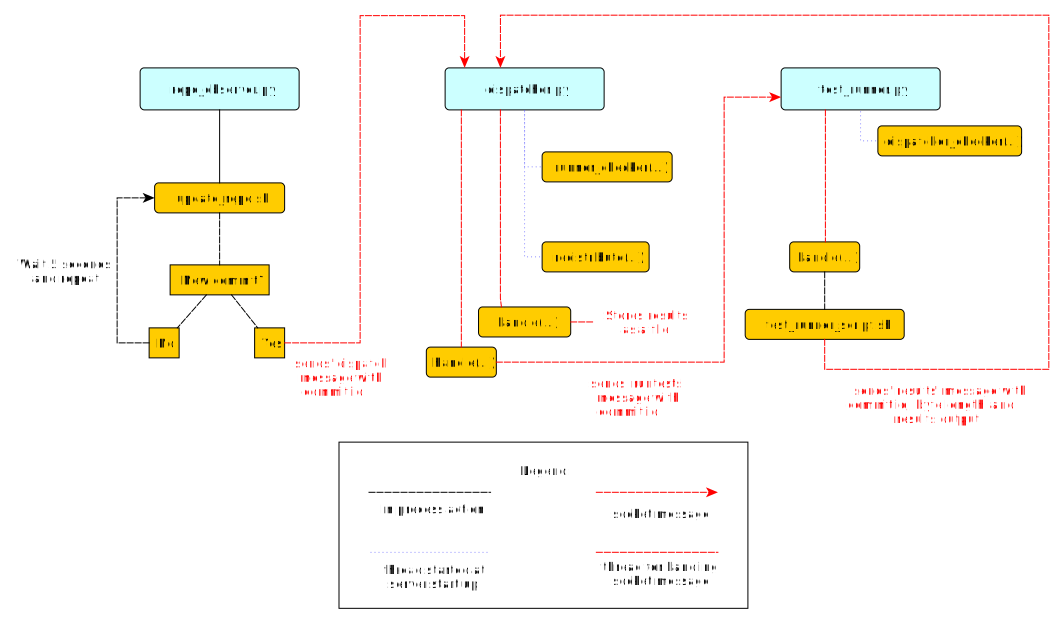
\includegraphics{diagram.svg}

\aosasectii{Running the Code}\label{running-the-code}

We can run this simple CI system locally, using three different terminal
shells for each process.

We start the dispatcher first, running on port 8888:

\begin{aosadescription}

\item[``]
\$ python dispatcher.py
\end{aosadescription}

\begin{center}\rule{3in}{0.4pt}\end{center}

In a new shell, we start the test runner (so it can register itself with
the dispatcher):

\begin{aosadescription}

\item[``]
\$ python test\_runner.py
\textless{}path/to/test\_repo\_clone\_runner\textgreater{}
\end{aosadescription}

\begin{center}\rule{3in}{0.4pt}\end{center}

The test runner will assign itself its own port, in the range 8900-9000.
You may run as many test runners as you like.

Lastly, in another new shell, let's start the repo observer:

\begin{aosadescription}

\item[``]
\$ python repo\_observer.py --dispatcher-server=localhost:8888
\textless{}path/to/test\_repo\_clone\_obs\textgreater{}
\end{aosadescription}

\begin{center}\rule{3in}{0.4pt}\end{center}

Now that everything is set up, let's trigger some tests! To do that,
we'll need to make a new commit. Go to your master repository and make
an arbitrary change:

\begin{aosadescription}

\item[``]
\$ cd /path/to/test\_repo \$ touch new\_file \$ git add new\_file \$ git
commit -m``new file'' new\_file
\end{aosadescription}

\begin{center}\rule{3in}{0.4pt}\end{center}

Then repo\_observer.py will realize that there's a new commit and notify
the dispatcher. You can see the output in their respective shells, so
you can monitor them. Once the dispatcher receives the test results, it
stores them in a test\_results/ folder in this code base, using the
commit ID as the filename.

\aosasecti{Error Handling}\label{error-handling}

This CI system includes some simple error handling.

If you kill the test\_runner.py process, dispatcher.py will figure out
that the runner is no longer available and will remove it from the pool.

You can also kill the test runner, to simulate a machine crash or
network failure. If you do so, the dispatcher will realize the runner
went down and will give another test runner the job if one is available
in the pool, or will wait for a new test runner to register itself in
the pool.

If you kill the dispatcher, the repository observer will figure out it
went down and will throw an exception. The test runners will also
notice, and shut down.

\aosasecti{Conclusion}\label{conclusion}

By separating concerns into their own processes, we were able to build
the fundamentals of a distributed continuous integration system. With
processes communicating with each other via socket requests, we are able
to distribute the system across multiple machines, helping to make our
system more reliable and scalable.

Since the CI system is quite simple now, you can extend it yourself to
be far more functional. Here are a few suggestions for improvements:

\aosasectii{Per-Commit Test Runs}\label{per-commit-test-runs}

The current system will periodically check to see if new commits are run
and will run the most recent commit. This should be improved to test
each commit. To do this, you can modify the periodic checker to dispatch
test runs for each commit in the log between the last tested commit and
the latest commit.

\aosasectii{Smarter Test Runners}\label{smarter-test-runners}

If the test runner detects that the dispatcher is unresponsive, it stops
running. This happens even when the test runner is in the middle of
running tests! It would be better if the test runner waited for a period
of time (or indefinitely, if you do not care about resource management)
for the dispatcher to come back online. In this case, if the dispatcher
goes down while the test runner is actively running a test, instead of
shutting down it will complete the test and wait for the dispatcher to
come back online, and will report the results to it. This will ensure
that we don't waste any effort the test runner makes, and that we will
only run tests once per commit.

\aosasectii{Real Reporting}\label{real-reporting}

In a real CI system, you would have the test results report to a
reporter service which would gather the results, post them somewhere for
people to review, and notify a list of interested parties when a failure
or other notable event occurs. You can extend our simple CI system by
creating a new process to get the reported results, instead of the
dispatcher gathering the results. This new process could be a web server
(or can connect to a web server) which could post the results online,
and may use a mail server to alert subscribers to any test failures.

\aosasectii{Test Runner Manager}\label{test-runner-manager}

Right now, you have to manually launch the test\_runner.py file to start
a test runner. Instead, you could create a test runner manager process
which would assess the current load of test requests from the dispatcher
and scale the number of active test runners accordingly. This process
will receive the runtest messages and will start a test runner process
for each request, and will kill unused processes when the load
decreases.

Using these suggestions, you can make this simple CI system more robust
and fault-tolerant, and you can integrate it with other systems, like a
web-based test reporter.

If you wish to see the level of flexibility continuous integration
systems can achieve, I recommend looking into
\href{http://jenkins-ci.org/}{Jenkins}, a very robust, open-source CI
system written in Java. It provides you with a basic CI system which you
can extend using plugins. You may also access its source code
\href{https://github.com/jenkinsci/jenkins/}{through GitHub}. Another
recommended project is \href{https://travis-ci.org/}{Travis CI}, which
is written in Ruby and whose source code is also available
\href{https://github.com/travis-ci/travis-ci}{through GitHub}.

This has been an exercise in understanding how CI systems work, and how
to build one yourself. You should now have a more solid understanding of
what is needed to make a reliable distributed system, and you can now
use this knowledge to develop more complex solutions.

\end{aosachapter}
